\documentclass[aspectratio=169, 12pt]{beamer}
% \documentclass[aspectratio=169, 12pt, handout]{beamer}

    \usetheme{metropolis}
    % \usepackage{myslides}
    \usepackage{bm}
    \usepackage{nicefrac}
    \usepackage{pgfplots}
    \pgfmathsetlengthmacro\MajorTickLength{
        \pgfkeysvalueof{/pgfplots/major tick length} * 0.5
    }
    \pgfmathsetlengthmacro\MinorTickLength{
        \pgfkeysvalueof{/pgfplots/minor tick length} * 0.5
    }

    \usepackage{tikz}
    \tikzset{every picture/.style={font issue=\small}, font issue/.style={execute at begin picture={#1\selectfont}}}
    \pgfplotsset{every axis/.append style={yticklabel style={font=\footnotesize}, xticklabel style={font=\footnotesize}}}
    \pgfplotsset{every axis/.append style={major tick length=\MajorTickLength, minor tick length=\MinorTickLength}}
    \pgfplotsset{every axis/.append style={legend style={font=\scriptsize, row sep=-1mm}}}
    \usepackage{tikzscale}
    \pgfplotsset{compat=newest}
    \pgfplotsset{plot coordinates/math parser=false}
    \usetikzlibrary{fit}
    \newlength\figwidth
    \newlength\figheight
     
    \usetikzlibrary{shapes.arrows}
    \usepackage{tabularx}


\title{Embedding collaborative practice in introductory programming courses}
% \date{Monday 12th December 2022}
\author{Charlotte Desvages}
\institute{School of Mathematics, University of Edinburgh, UK}

% \titlegraphic{\includegraphics[width=0.8\textwidth]{figures/AAGlogo_wide.PNG}\includegraphics[width=0.18\textwidth]{figures/ICSV26-logo.jpg}}

\begin{document}

\maketitle

% \begin{frame}{Outline}
    % \begin{itemize}
        % \item Background: computer labs in SoM before 2020
        % \item The catalyst: teaching online
        % \item Pair programming in computer labs
        % \item Peer-assessed code review
        % \item How did it go?
    % \end{itemize}
% \end{frame}

\section{Background: Computing labs in the School of Maths}
\setbeamercovered{transparent}

\begin{frame}{Background: Computing labs in the School of Maths}
    \begin{itemize}
        \item<1-> Computing courses from Y1 to MSc, most are taught in either Python or R.
        \item<2-> Topics include numerical analysis, statistics, data science, machine learning, optimisation\ldots
        \item<3-> Many courses run \textbf{drop-in} computer labs: students come sit in the lab and work through exercises, tutors walk around the room to check in and help.
        \item<4-> Typically, during a lab, pairs and triples form organically as students sit next to friends.
    \end{itemize}
\end{frame}

% \begin{frame}{Moving online: Summer 2020}
    % \begin{itemize}
        % \item<1-> \textit{Problem:} computer labs (with shared dirty keyboards!) are not an optimal use of our teaching spaces for hybrid, socially-distanced teaching.

            % $\rightarrow$ Early decision: all our computer labs will be \textbf{fully online}.

        % \item<2-> \textit{New problem:} keeping students engaged can be more difficult in online courses, and our students are not used to distance learning.

            % $\rightarrow$ the ``passive'' drop-in lab is clearly not the best use of our limited contact time with the students.

    % \end{itemize}
    % \pause
    % \pause
    % Having to rethink course delivery provided an opportunity to refresh the syllabus and rethink \textbf{learning outcomes}, to emphasise good programming practice and familiarise students with standard workflows.
% \end{frame}

\begin{frame}{Combining collaborative learning and good practice}
    How can I promote peer learning and effective collaboration in an online programming class?
    \begin{enumerate}
        \item<1-> Synchronous:
            \begin{itemize}
                \item \textbf{Pair programming} in problem-based labs
                \item Live coding in lectures (``collaborative learning'' with the lecturer)
                \item Small group peer code review
            \end{itemize}
        \item<2-> Asynchronous:
            \begin{itemize}
                \item Discussion board (Piazza)
                \item \textbf{Peer-assessed code review} task
            \end{itemize}
    \end{enumerate}
\end{frame}

\begin{frame}{Cohorts}
    Pair programming and peer-assessed code reviews deployed in two courses:
    \begin{itemize}
        \item<1-> Semester 1: \textbf{Python Programming} (MSc, 250 students). Introductory Python course, focused on programming skills, overviewing some applications in applied maths and data science.
        \item<2-> Semester 2: \textbf{Computing and Numerics} (Y2, 250 students). Introductory Python course, but learning outcomes focused on computational mathematics and numerical methods.
    \end{itemize}
\end{frame}

\section{Pair programming as a pedagogical tool}

\begin{frame}{The pair programming workflow}
    \centering
    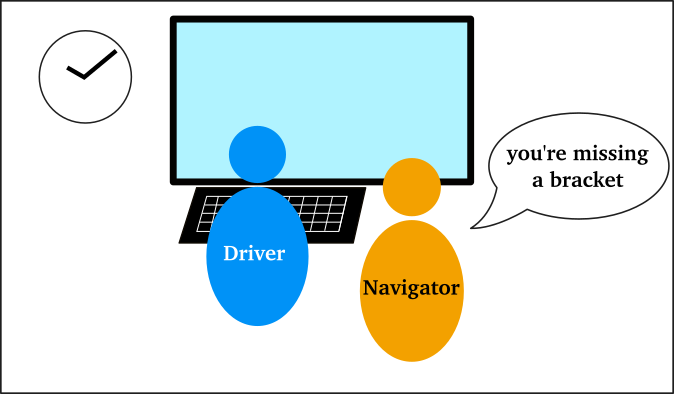
\includegraphics[width=0.8\textwidth]{graphics/pairprog_1.png}
\end{frame}

\begin{frame}{The pair programming workflow}
    \centering
    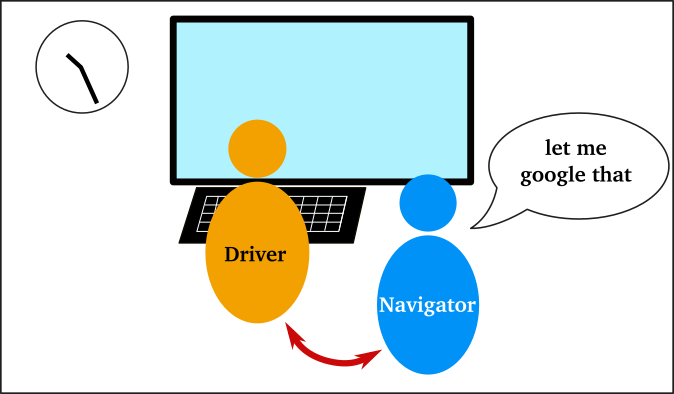
\includegraphics[width=0.8\textwidth]{graphics/pairprog_2.png}
\end{frame}

\begin{frame}{Motivations for trying pair programming}
    \begin{itemize}
        \item<1-> \textbf{Small groups} (2 or 3): all students take an active role in solving the task, (have to) talk to each other.
        \item<2-> \textbf{Structured/scripted roles}: less time and cognitive effort spent on figuring out a way to collaborate efficiently/productively (``unscripted'' collaboration can be particularly unnatural to navigate in a virtual ``room'').
        \item<3-> Tutors can't always ``keep an eye'' on the whole room and identify who needs help: working in pairs gives everyone an \textbf{immediately accessible source of help}, minimises tutor time spent on ``trivial'' mistakes (syntax errors, typos\ldots).
        \item<4-> Introducing standard \textbf{professional practice}.
    \end{itemize}
\end{frame}

\section{Distributed/remote pair programming}

\begin{frame}{Session organisation}
    \centering
    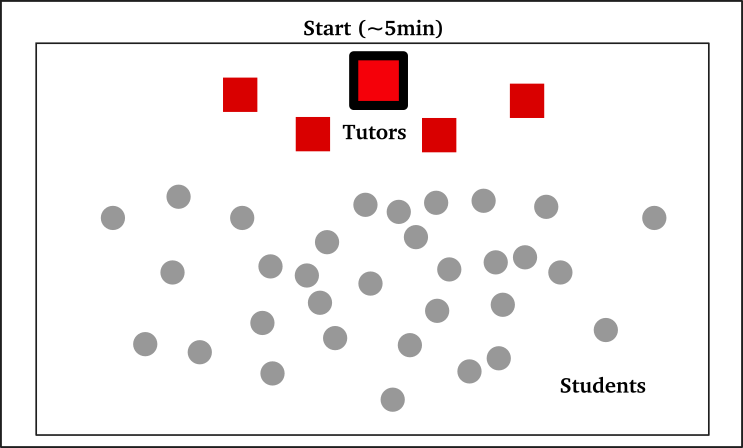
\includegraphics[width=0.7\textwidth]{graphics/pairprog_3.png}
\end{frame}

\begin{frame}{Session organisation}
    \centering
    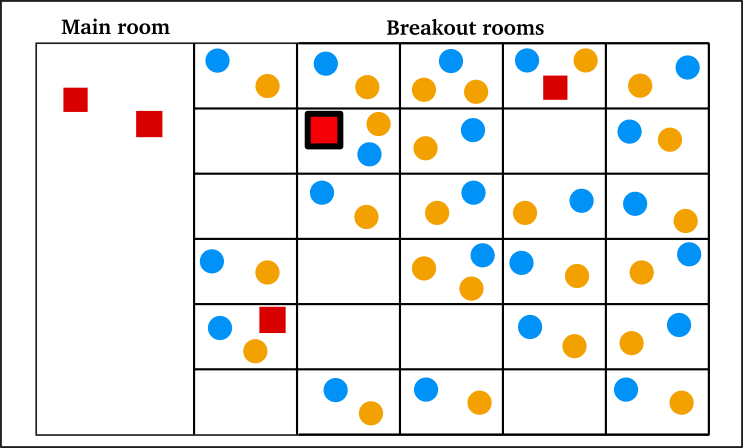
\includegraphics[width=0.7\textwidth]{graphics/pairprog_4.png}
\end{frame}

\begin{frame}{Inside a breakout room}
    \begin{center}
    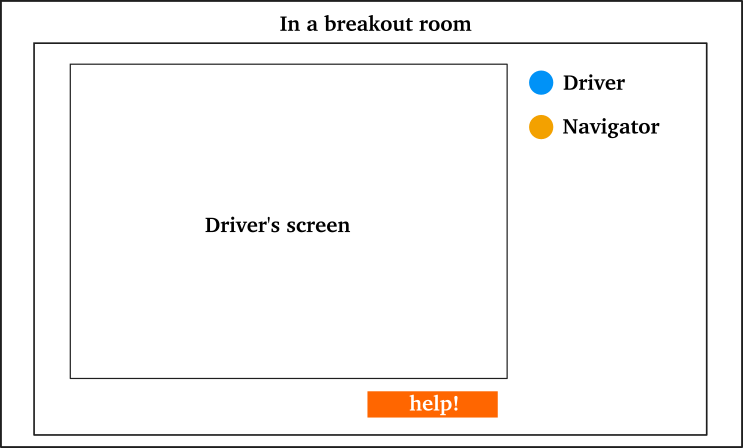
\includegraphics[width=0.7\textwidth]{graphics/pairprog_5.png}
    \end{center}
\end{frame}

\begin{frame}{Inside a breakout room}
    \begin{enumerate}
        \item Driver \textbf{forks} a template GitHub repo containing the task; navigator joins the forked repo (easily set up with GitHub Classroom).
        \item Driver \textbf{clones} the repo, shares their screen, and starts working on the task.
        \item Navigator reads instructions, actively observes, talks to the driver, checks documentation\ldots
        \item They \textbf{switch roles} after $\sim$15 minutes. Old driver commits and pushes their changes, new driver pulls, shares their screen, and continues.
    \end{enumerate}
\end{frame}

\begin{frame}{Getting help}
    \centering
    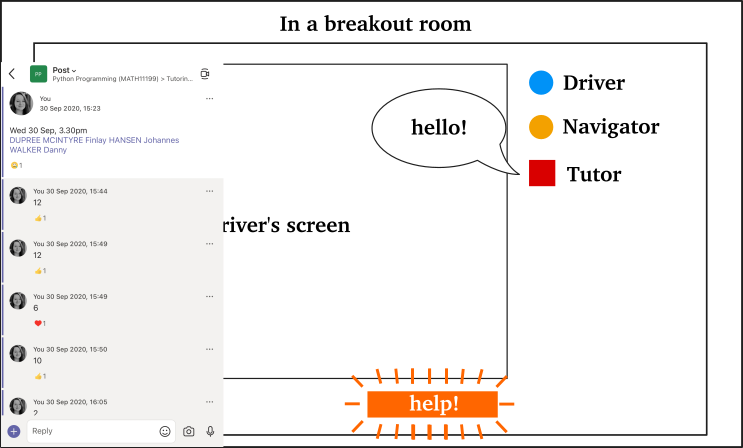
\includegraphics[width=0.7\textwidth]{graphics/pairprog_6.png}
\end{frame}

\section{How did it go?}

\begin{frame}{Student feedback: the positives}
    \begin{center}
    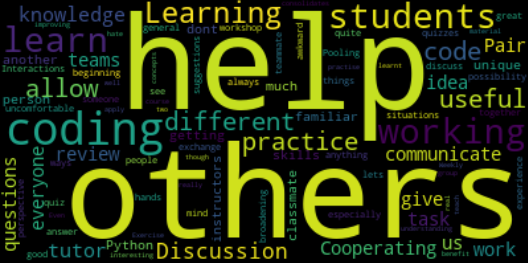
\includegraphics[width=0.5\textwidth]{graphics/workshops_feedback_positive.png}

    ``What do you consider to be the most useful aspects of the workshops?''
    \end{center}
    \pause

    \begin{itemize}
        \item Most of the responses point at cooperation, discussion, peer learning as positive aspects.
        \item Other positive comments: the workshop tasks are interesting, I get to apply the skills I've learned, I can get good help from tutors.
    \end{itemize}
\end{frame}

\begin{frame}{Student feedback: the positives}
    Some representative comments heard/read from students:
    \begin{itemize}
        \item ``This is the most 'social' course I have'' / ``This workshop is my main social interaction for the week''
        \item ``I didn't interact much with tutors since we often solved coding issues by ourselves. This is a good feature of the workshop.''
        \item ``[Workshops] allow you to have interaction with other students and help from tutors at the same time.''
        \item ``It was good to meet people and learn to pair program.''
        \item ``Peer (sic) programming is great. I'm not sure if this was a new addition to the course or not, but I hope it stays.''
        \item ``Working with others is also a real benefit as it allows you to learn from others, or teach others which further consolidates your own learning.''
    \end{itemize}
\end{frame}

\begin{frame}{Student feedback: the negatives}
    \begin{itemize}
        \item<1-> Most of the negative feedback on \textbf{pair programming labs} mentions the lack of time -- 1 hour was too short.
        \item<2-> Some friction with technical issues, complicated workflow with git/GitHub/IDE for beginners, particularly at the start of the semester. This improved as the students got used to their tools.
        \item<3-> Some issues with \textbf{incompatible pairs}.
    \end{itemize}
\end{frame}

\begin{frame}{Student feedback: the negatives}
    Some ad-hoc comments heard/read from students:
    \begin{itemize}
        \item ``I didn't like the format (work in pairs) so I decided not to go to many of them.''
        \item ``There are a lot of tasks for the short time of the workshops usually. Also pair programming online is sometimes just watching another person googling something, so I'm not really sure if Pair Programming is the way to go for the workshops.''
        \item ``I found [the workshops] useful when I found a good group of people to work with.''
        \item ``Too much work not enough time. I would have benefited from a two hour workshop instead.''
    \end{itemize}
\end{frame}


\begin{frame}{Incompatible pairs}
    As a ``non-specialist'' cohort, levels of programming experience (and even general computer literacy) vary immensely between the students coming into the course. Dysfunctional pairs were typically:
    \begin{itemize}
        \item very experienced + complete beginner (a frustrating experience for both),
        \item two complete beginners (got stuck very easily).
    \end{itemize}
    \pause

    Zoom update in Autumn 2020 allowed attendees to choose their own breakout rooms. Issues with mismatched pairs and lack of confidence from beginners were greatly reduced by:
    \begin{itemize}
        \item letting students choose their pair (so they could work with a friend),
        \item letting students work in triples instead of pairs, with a rotating driver and two navigators.
    \end{itemize}
\end{frame}


\section{Changes from 2021}
\begin{frame}{Pair programming in the classroom}
    Broadly the same workflow!
    \begin{itemize}
        \item Students work from their own laptops.
        \item Students work in groups of 2 or 3. They choose who they work with.
        \item GitHub still used for sharing work; students are reminded to change roles every 15-20 minutes.
        \item From this year: GitHub Codespaces as a cloud computing environment (for now, free for teaching) --- no need to install anything!
    \end{itemize}
\end{frame}

\begin{frame}{Pair programming in the classroom}
    \begin{itemize}
        \item Easier to tutor!
        \item Student feedback still very positive.
        \item 2022: back to 2-hour workshops.
            \begin{itemize}
                \item Tasks were kept the same as for the 1-hour workshops.
                \item ``Further work'' was attempted by a lot more students.
                \item Much fewer complaints about technical issues or having too little time.
            \end{itemize}
    \end{itemize}
\end{frame}

\section{Peer-assessed code review}

\begin{frame}{Motivations for peer code review}
    \begin{itemize}
        \item<1-> \textbf{Peer learning} by seeing how others have approached the same task.
        \item<2-> Building \textbf{good habits}: students are asked to assess robust testing, commenting and style, code structure\ldots
        \item<3-> Helping to build a sense of \textbf{community}: students don't have as much opportunity to work and learn together.
        \item<4-> Introducing \textbf{standard professional practice}.
        \item<5-> Better understanding of the assessment process.
    \end{itemize}
\end{frame}

\begin{frame}{Planning: 2020}
    \begin{itemize}
        \item<1-> Code review tasks were alternating with quizzes as weekly homework (5-10\% total grade).
        \item<2-> Set over 2 weeks: submit your solution by the end of the first week, peer-assess 3 submissions by the end of the second week.
        \item<3-> In code review weeks, the \textbf{synchronous lab} was a small group scaffolding + peer review activity:
            \begin{itemize}
                \item Peer review only was not particularly successful. Students would be finished in quite a short time, and the submissions they had to actually assess were not those from their discussion group.
                \item Starting the activity with a scaffolding task was helpful: e.g. a debugging task to practice understanding error traces and troubleshooting, a discussion task on useful commenting and code style. As seen with pair programming, \textbf{structure helps!}
            \end{itemize}
    \end{itemize}
\end{frame}

\begin{frame}{Setup using Moodle Workshop}
    \begin{itemize}
        \item<1-> I used the \textbf{Moodle Workshop plugin}, built for peer-assessed tasks.
            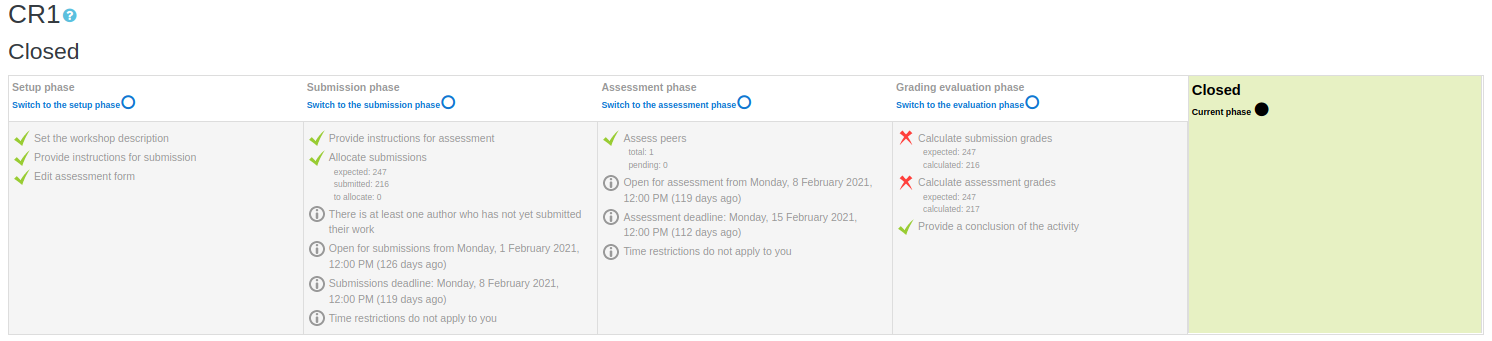
\includegraphics[width=0.8\textwidth]{graphics/workshop.png}
        \item<2-> The grade is calculated as 50\% peer-assessed, and 50\% for \textit{how close} your assessment was to the consensus between the 3 reviewers.
        \item<3-> The task description included the problem specification, instructions for submission format, and marking scheme to be used.
    \end{itemize}
\end{frame}


\begin{frame}{Setup using Moodle Workshop}
    \textbf{Moderation}:
    \begin{itemize}
        \item As instructor, I could override grades, add my own assessment, or change weights of different assessments.
        \item I checked a sample of random submissions/assessments each week.
        \item I set up a form which students could use to request further instructor moderation.
    \end{itemize}
\end{frame}



\begin{frame}{Peer-assessed code reviews}
    Based on student feedback (workload, scaffolding, workshop discussions):
    \begin{itemize}
        \item Submit \textbf{solution to quiz question} for peer-assessment.
            \begin{itemize}
                \item Much less added workload (assuming the quiz is completed).
                \item Burden of assessing \textbf{correctness} is taken away from students.
                \item Focus on readability, commenting, structure, efficiency.
            \end{itemize}
        \item Provide \textbf{instructor-assessed examples} to go through before peer assessment.
            \begin{itemize}
                \item Provides an element of self-assessment/calibration before peer assessment.
                \item Provides examples of what constructive feedback looks like.
                \item Provides opportunity to highlight common shortcomings.
            \end{itemize}
    \end{itemize}
\end{frame}

\section{Final thoughts}

\begin{frame}{Final thoughts}
    Overall, pair programming was a success in fostering productive \textbf{cooperation} and \textbf{peer-learning} in an online setting, \textit{for students who attended}. The main issues were around time and pairing compatibility.
    \pause

    With sufficient scaffolding and robust moderation, peer-assessed code review has also been well-received and helpful to get students to think more carefully about \textbf{good practice in programming}.
\end{frame}

\begin{frame}{Communities of practice}
    \textbf{Pair programming club} has been meeting up regularly since the summer.

    We're an informal group of lecturers and tutors teaching programming labs in a wide range of disciplines at the University of Edinburgh (for now!). We meet together to try different ways to pair-program, to discuss how it works in our respective courses, and to address specific questions and challenges.

    There are \textbf{many different ways} (and tools) to set up pair programming in your classroom.

    There is no commitment -- join whenever you want if you're interested in trying pair-programming!
\end{frame}



\end{document}
